\chapter{Handling of trimuon correlations at LHCb}
\label{chap:trimuon}

\textit{Having three muons passing through the detector may result in few issues. Two collimated muons may be passing through the same parts of the detector if they bear the same charge, which causes problems in resolving them. From tracking point of view, ghosts and clones are hence much more likely to occur. In LHCb, plethora of muon \Gls{PID} variables can be used to suppress these spurious tracks, however, one must be careful once estimating the relevant \gls{PID} efficiencies as most these efficiencies will be dependant on number of muons in the detector.}

\section{Binary Muon PID variables}
There is a further set of muon variables apart from the ones mentioned in \autoref{muonID} that are avialable for \gls{PID} of muon. Similar to \texttt{isMuon} there are two more binary variables, \texttt{isMuonTight} and \texttt{isMuonLoose}, that can help with classification of muons. 

In each station (M1-M4) and in each dimension, $d=$(x or y), \gls{FOI} is defined as a function of momentum $p$,
\begin{equation}
	FOI_{d}=\rho_{d,1}+\rho_{d,2}\cdot \exp \left(\frac{\rho_{d,3}\cdot p}{\gevc} \right).
\end{equation}

Muon passing through the detector will leave hit in $pad_{d}$ of each muon station and have $h_{d}$ coordinate. Extrapolations from tracking system are made into the stations are denoted $E_{d}$. The hits are considered to be within the \gls{FOI} for given $d$ if $|| h_{d} - E_{d} || < FOI_{d} \cdot pad_{d}$. 

Because the detector information is read out in $x$ $y$ direction separately, the pad slicing according to read-out is known as \textit{physical} slicing of pads. However, as seen in \autoref{fig:pads}, the overlapping \textit{physical} pads are grouped into \textit{logical} pads. Uncrossed hits are registered within \textit{physical} pads only and crossed hits are given by \textit{logical} pads. \texttt{isMuon} only requires positive decision from uncrossed hits, whereas \texttt{isMuonTight} requires crossed hits. 


\begin{figure}[!h]
        \centering
        %
\includegraphics[width = 0.3\textwidth]{figs/trimuon/poze.jpg}
        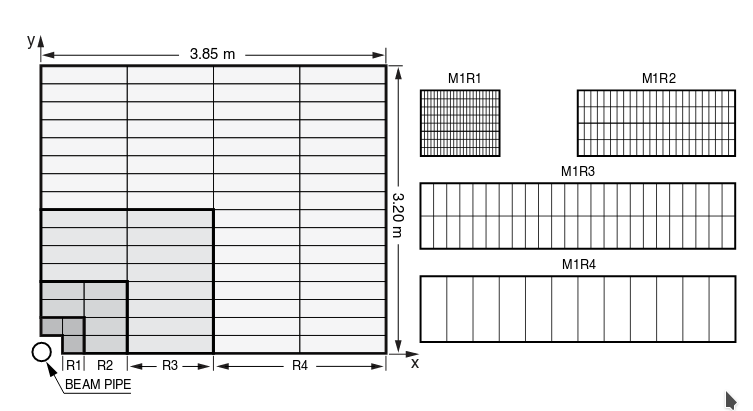
\includegraphics[width = 1.0\textwidth]{figs/trimuon/pad.png}
        \caption{Schematic view of the muon station slicing into x-y pads. This is left quadrant of M1 station, showing decreasing granularity of the muon stations away from the beam. This figure has been taken from \cite{LHCb-DP-2012-002}. M1R1 is the innermost region and M1R4 is the outermost region of the M1 station. }
        \label{fig:pads}
\end{figure}

\section{Muon PID variables based on sharing hits}
\label{bugs}

The \texttt{nShared} variable for muons gives number of tracks with shared hits in the muon stations. For each hit within \gls{FOI} of the extrapolated track, the \texttt{nShared} algorithm will check whether any other track has been established using the given hit. In this case, the muon track which has bigger distance between the extrapolation and the hit is increased by 1 and the other tracks becomes the hit owner track. Hence this integer \gls{PID} variable, \texttt{nShared}, can help greatly reduce \textit{ghost} tracks and \textit{clones} if \texttt{nShared==0}.

\subsection{Different \texttt{nShared} definitions for Run \Rn{1} and Run \Rn{2}}
To make sure that muons for \Bmumumu are not coming from these spurious tracks,  \texttt{nShared==0} for all three muons, i.e, not to share hits in muon stations with any other downstream or long tracks. In analysing data, there were features in the software which changed between Run \Rn{1} and Run \Rn{2}.

The first feature that is different comes from the calculation of the distance between the extrapolation and the hit in \texttt{nShared} algorithm.
In \textit{Stripping 21} used for 2012 and \textit{21r1} used for 2011 data, it was discovered that the distance between extrapolated track and hit was wrongly calculated, and hence this was corrected before \textit{Stripping 23}, used for 2015 data. Additionally, information from M1 station was used to calculate distances, even though M1 information is not usually used for muon ID algorithm.  For analysts, this feature was present accross all reconstruction software and hence it is consistent within stripping version, meaning that simulation and data is affected in the same way.

In \textit{Stripping 23}, the Muon ID alghorithm was rewritten to adapt for parallelisation that needs to be done in order to meet criteria for upgrade of \gls{LHCb}. There were two mistakes introduced prior to 2015 datataking.
Firstly, an array was defined with 4-elements $[0,3]$ to store information about $x$ and $y$ coordinates of the hits. However, an iteration occured by filling $[1,4]$ array (M2-M5 station) resulting in 5-element array where 0-th element was not filled randomnly filled. However it turns out that it is well-behaved and has no impact on physics.

Futher in the process, however, this information is used to calculate the sum and average of distances per station between the hits and extrapolations. This algorithm again iterates over $[0,3]$ arrays, meaning that no information is used from M5 muon station. This obviously has effect, but again it is consistent accross the reconstruction version.

%\newline Summary of these features can be found in \href{https://indico.cern.ch/event/612764/contributions/2567244/attachments/1449649/2234804/20170426\_nShared.pdf}{\color{blue} in this presentation} 
The interplay between all these features for \bjpsimumuk can be seen in Figure~\ref{fig:nSharedvar}.

\begin{figure}[h!]
\centering
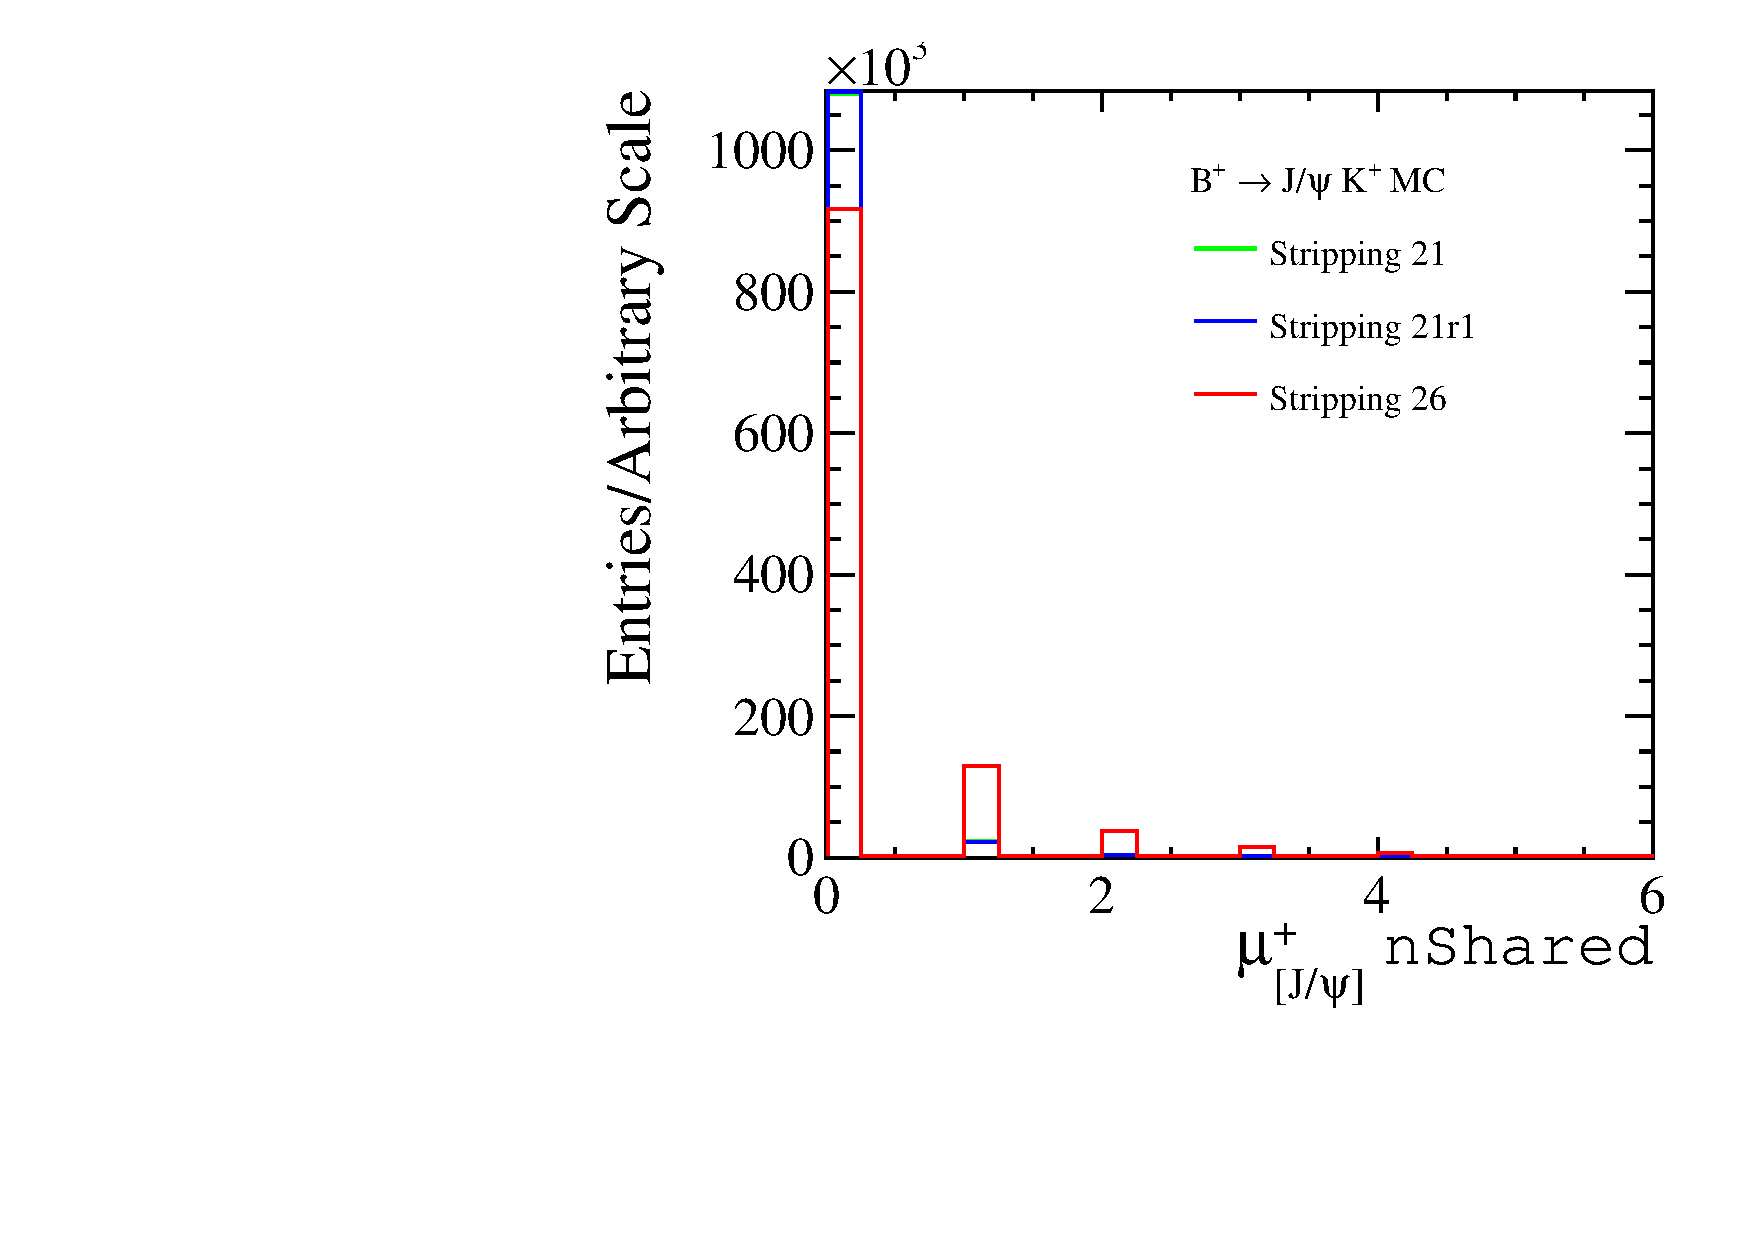
\includegraphics[width=0.5\linewidth]{trimuon/plotvariablemu1_nSharedJPSIKMC.pdf}\put(-40,133){(a)}
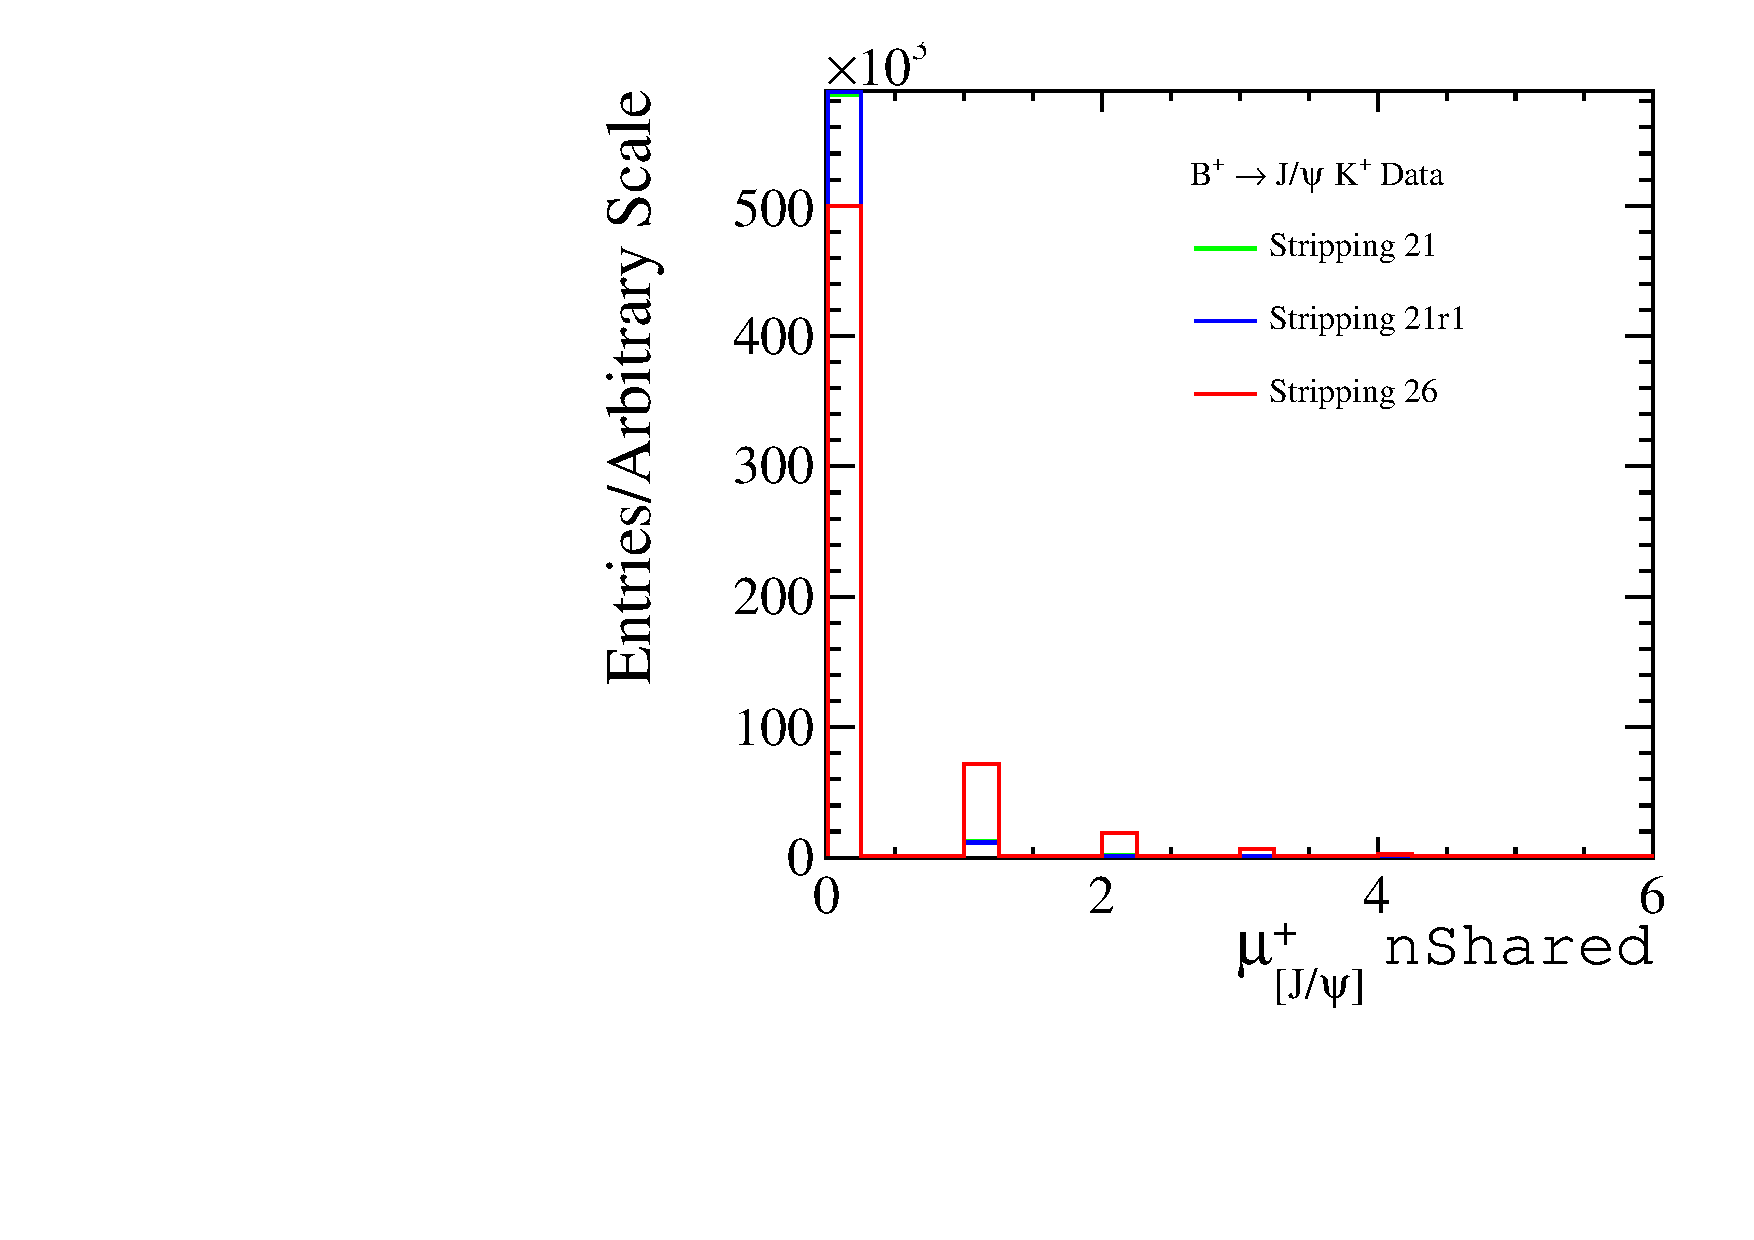
\includegraphics[width=0.5\linewidth]{trimuon/plotvariablemu1_nSharedJPSIKDATA.pdf}\put(-40,133){(b)}
	\caption{ (a) The \texttt{nShared} variable in simulation, (b) data for \bjpsimumuk in different stripping versions corresponding to 2012 (\textit{Stripping 21}), 2011 (\textit{Stripping 21r1}), 2016 (\textit{Stripping 26}) data-taking. There is shift of distribution in \textit{Stripping 26} towards less isolated tracks.}
\label{fig:nSharedvar}
%\vspace*{-1.0cm}
\end{figure}


This will have inevitably and impact on the \gls{PID} probabilities. Using the same calibration channels as in \autoref{muonperf}, misID and ID rates can be seen in Figure~\ref{fig:nSharedRun1andRun2}. As the tracks tend to be less isolated in \textit{Stripping 26}, typical of non-signal like events, the misID rate is expected to be higher for the same working point (ID efficiency).

\begin{figure}[h!]
\centering
%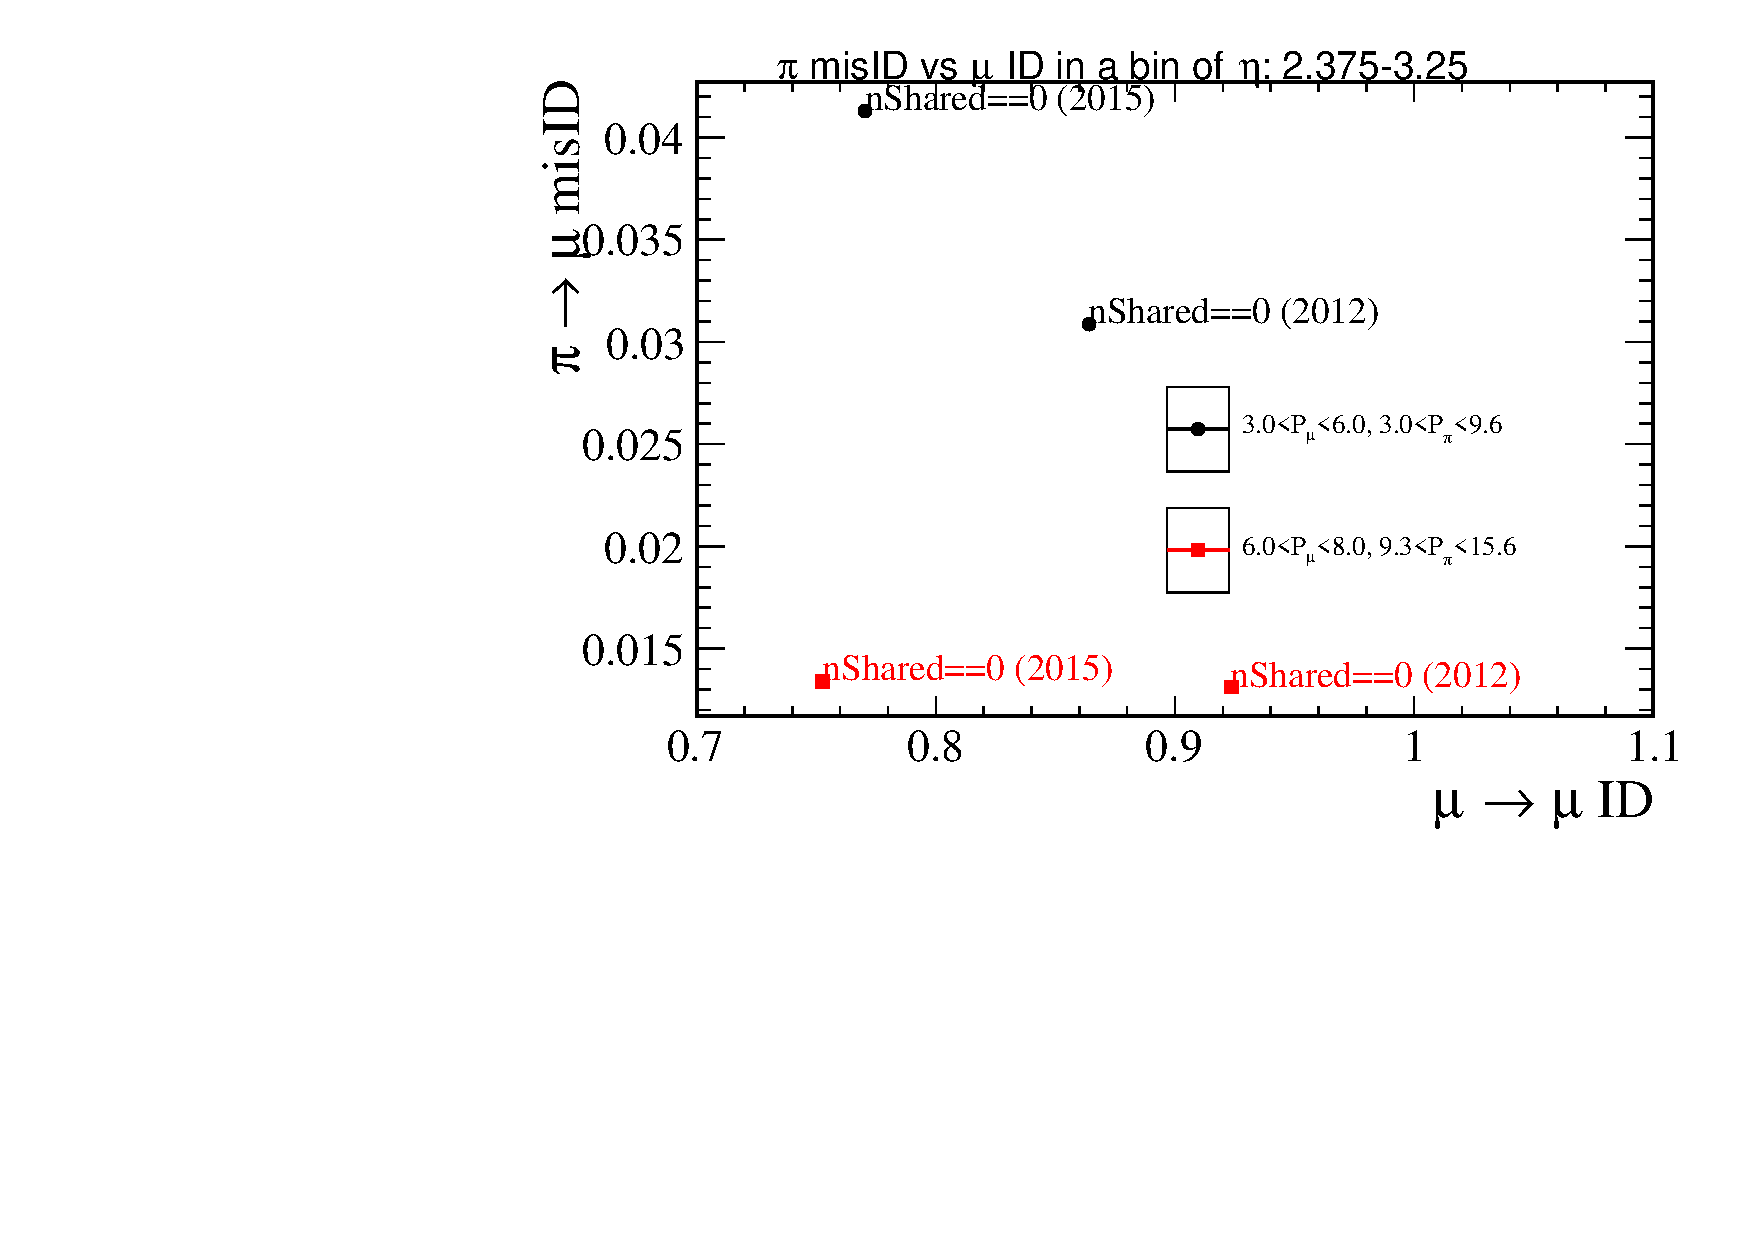
\includegraphics[width=0.52\linewidth]{compareRun1and2016selection/final_comparedirectly2012vs2015_nolog.pdf}%
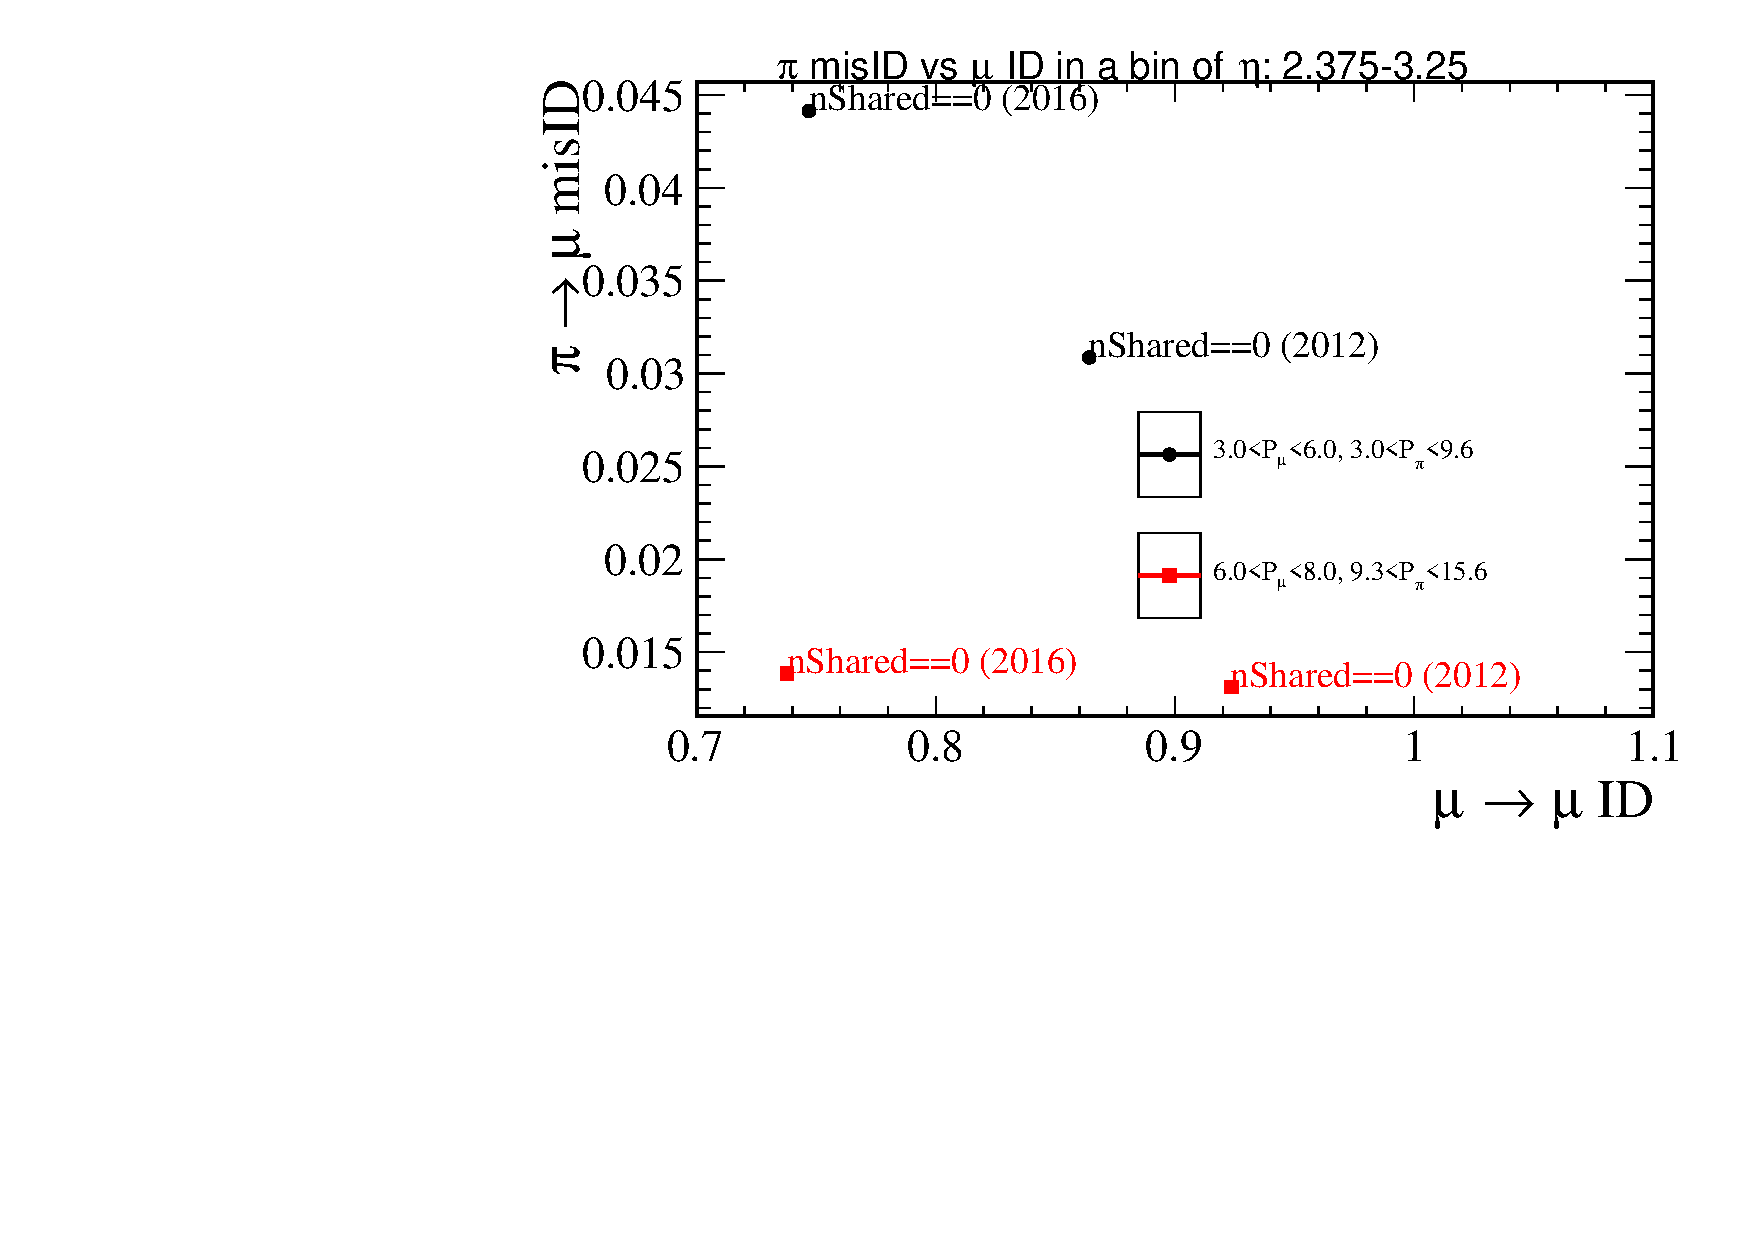
\includegraphics[width=0.7\linewidth]{trimuon/final_comparedirectly2012vs2016_nolog.pdf}
	\caption{ID and misID probabilities from standard calibration datasets from 2012 (\textit{Stripping 21}) 2016 (\textit{Stripping 26}), binned using default 2-dimensional binning scheme in momentum $p$ and pseudorapidity $\eta$. In this plot, ID and misID rate in central bin of $\eta$ and first and second bin in $p$ are compared. This demonstrates that for same ID efficiency, the misID rate is significantly higher in 2016.}
\label{fig:nSharedRun1andRun2}
%\vspace*{-1.0cm}
\end{figure}

\section{Muon PID variables based on regression techniques}
Similar to the $DLLmu$ variable in \autoref{muonID}, which combines all the information from the detector into a global likelihood, it is posible to feed all the different variables to a neural network, which can then produce an output 
corresponding to the probability of a particle to be of a certain species. \texttt{Probnn$\_{x}$} where, x is the species of interest, is calculated and can be used also for muonID. Compared to $DLL_{x}$ variables, \texttt{Probnn$\_{x}$} variables tend to have smaller correlation with the kinematics of the particle, and hence are more useful with decays where particles are soft, such as \Bmumumu. As with any machine learning alghotritms, the selection of the training sample is important as well as input variables. In \Rn{1} there were two tunings introduced \texttt{V2} and \texttt{V3}, with more variables in \texttt{V2}. Depending on the species of particles, \texttt{V2} or \texttt{V3} perfomed better.In the analysis of \Bmumumu \texttt{Probnn$\_${x}$\_$V2} is used.






%\newline In order to keep the signal efficiency high in 2016 data, as shown in Table ~\ref{tab:Reason}, softer condition ,$\texttt{nShared}<2$, is applied.


